% Please make sure you insert your
% data according to the instructions in PoSauthmanual.pdf
\documentclass{PoS}

\title{Rare decays at CMS}

\ShortTitle{Rare decays at CMS}

\author{\speaker{J\'onatan Piedra}\thanks{On behalf of the CMS Collaboration.}\\
        IFCA (CSIC - Universidad de Cantabria)\\
        E-mail: \email{piedra@cern.ch}}

%\author{Another Author\\
%        Affiliation\\
%        E-mail: \email{...}}

\abstract{..........................\
          ...........................}

\FullConference{XIV International Conference on Heavy Quarks and Leptons (HQL2018)\\
		May 27 - June 1, 2018\\
		Yamagata Terrsa, Yamagata, Japan}


\begin{document}


%-------------------------------------------------------------------------------
\section{Introduction}
%-------------------------------------------------------------------------------

To be filled.


%-------------------------------------------------------------------------------
\section{FCNC in ${\rm tZq \to 3\ell}$}
%-------------------------------------------------------------------------------

The source is~\cite{top-17-017}.
As can be seen in Figure~\ref{fig:TOP-17-017_Figure_003}.
As can be seen in Figure~\ref{fig:TOP-17-017_Figure_007}.


\begin{figure}[htb]
\centering
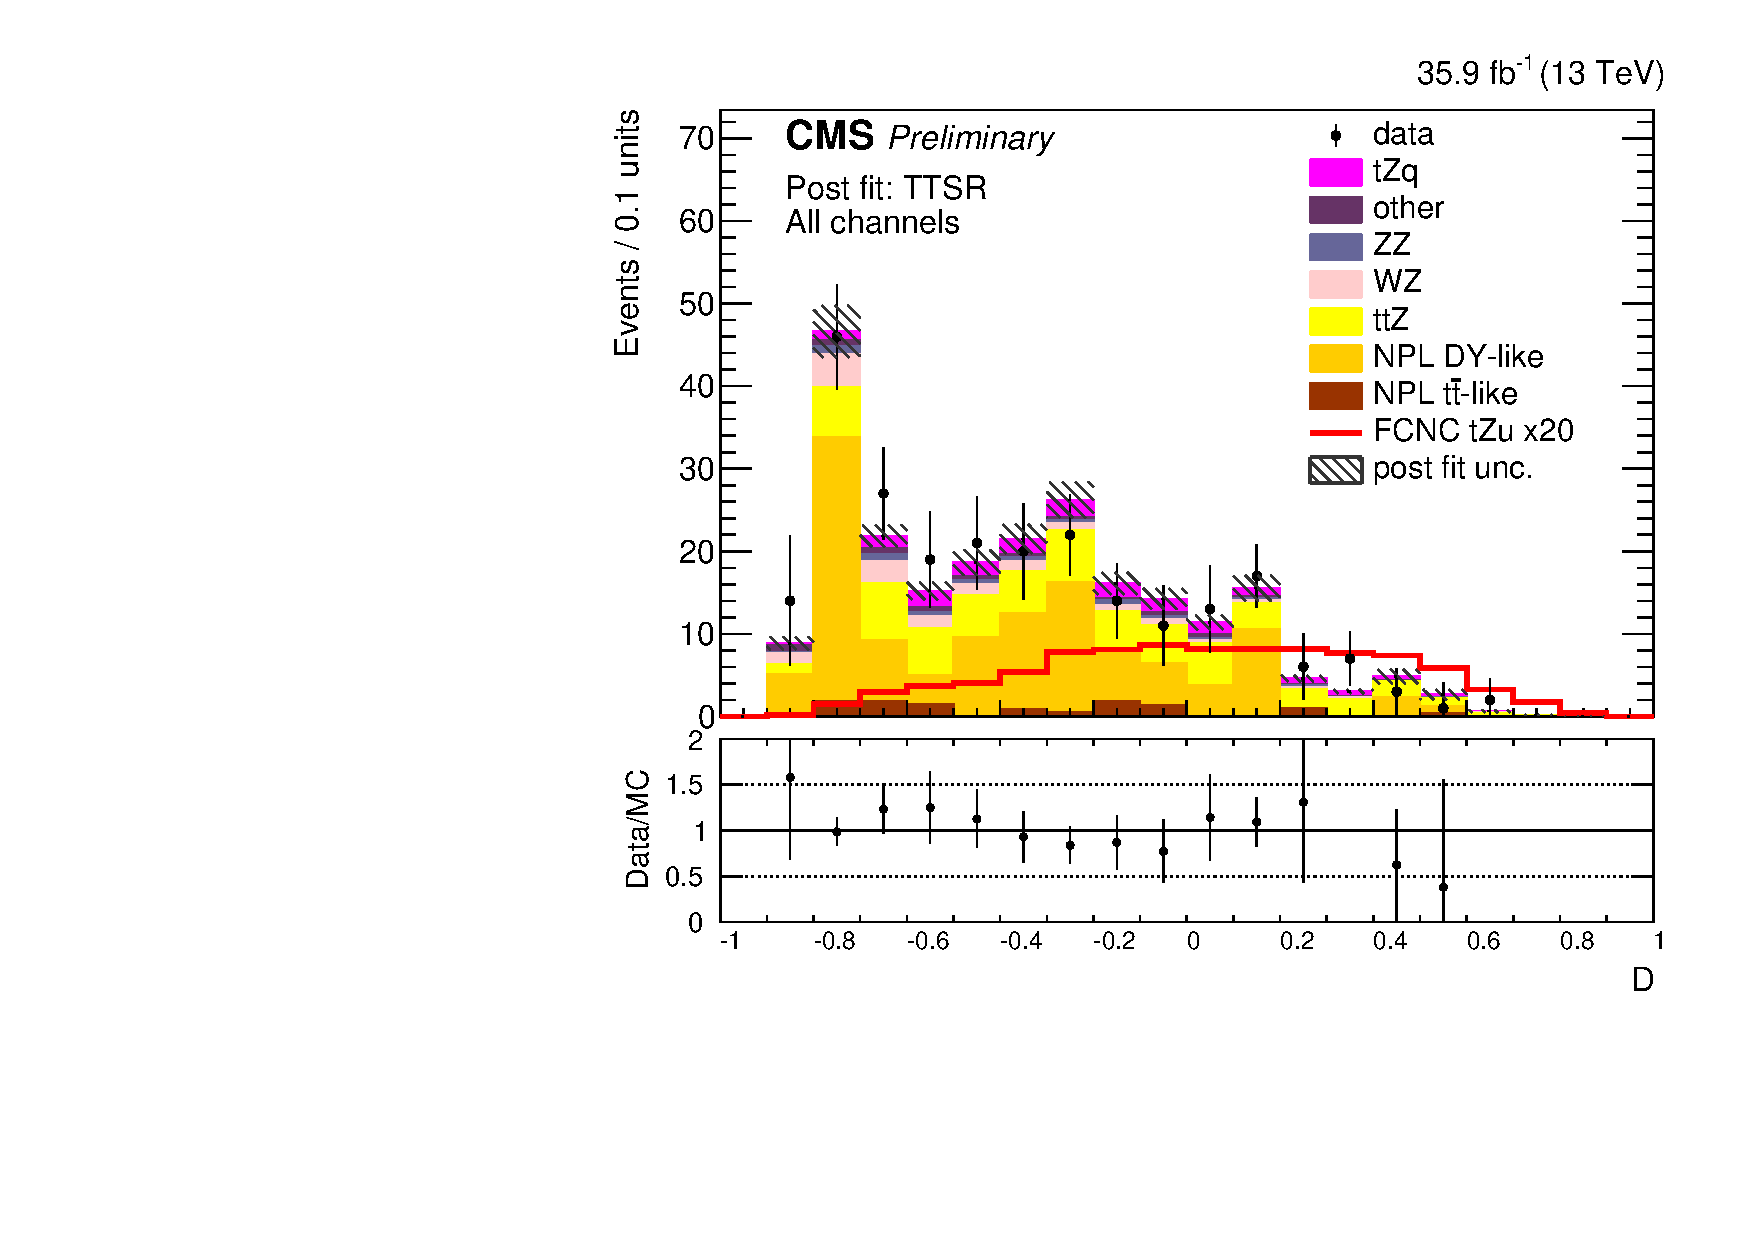
\includegraphics[width=0.45\textwidth]{figures/CMS-PAS-TOP-17-017_Figure_003-a}
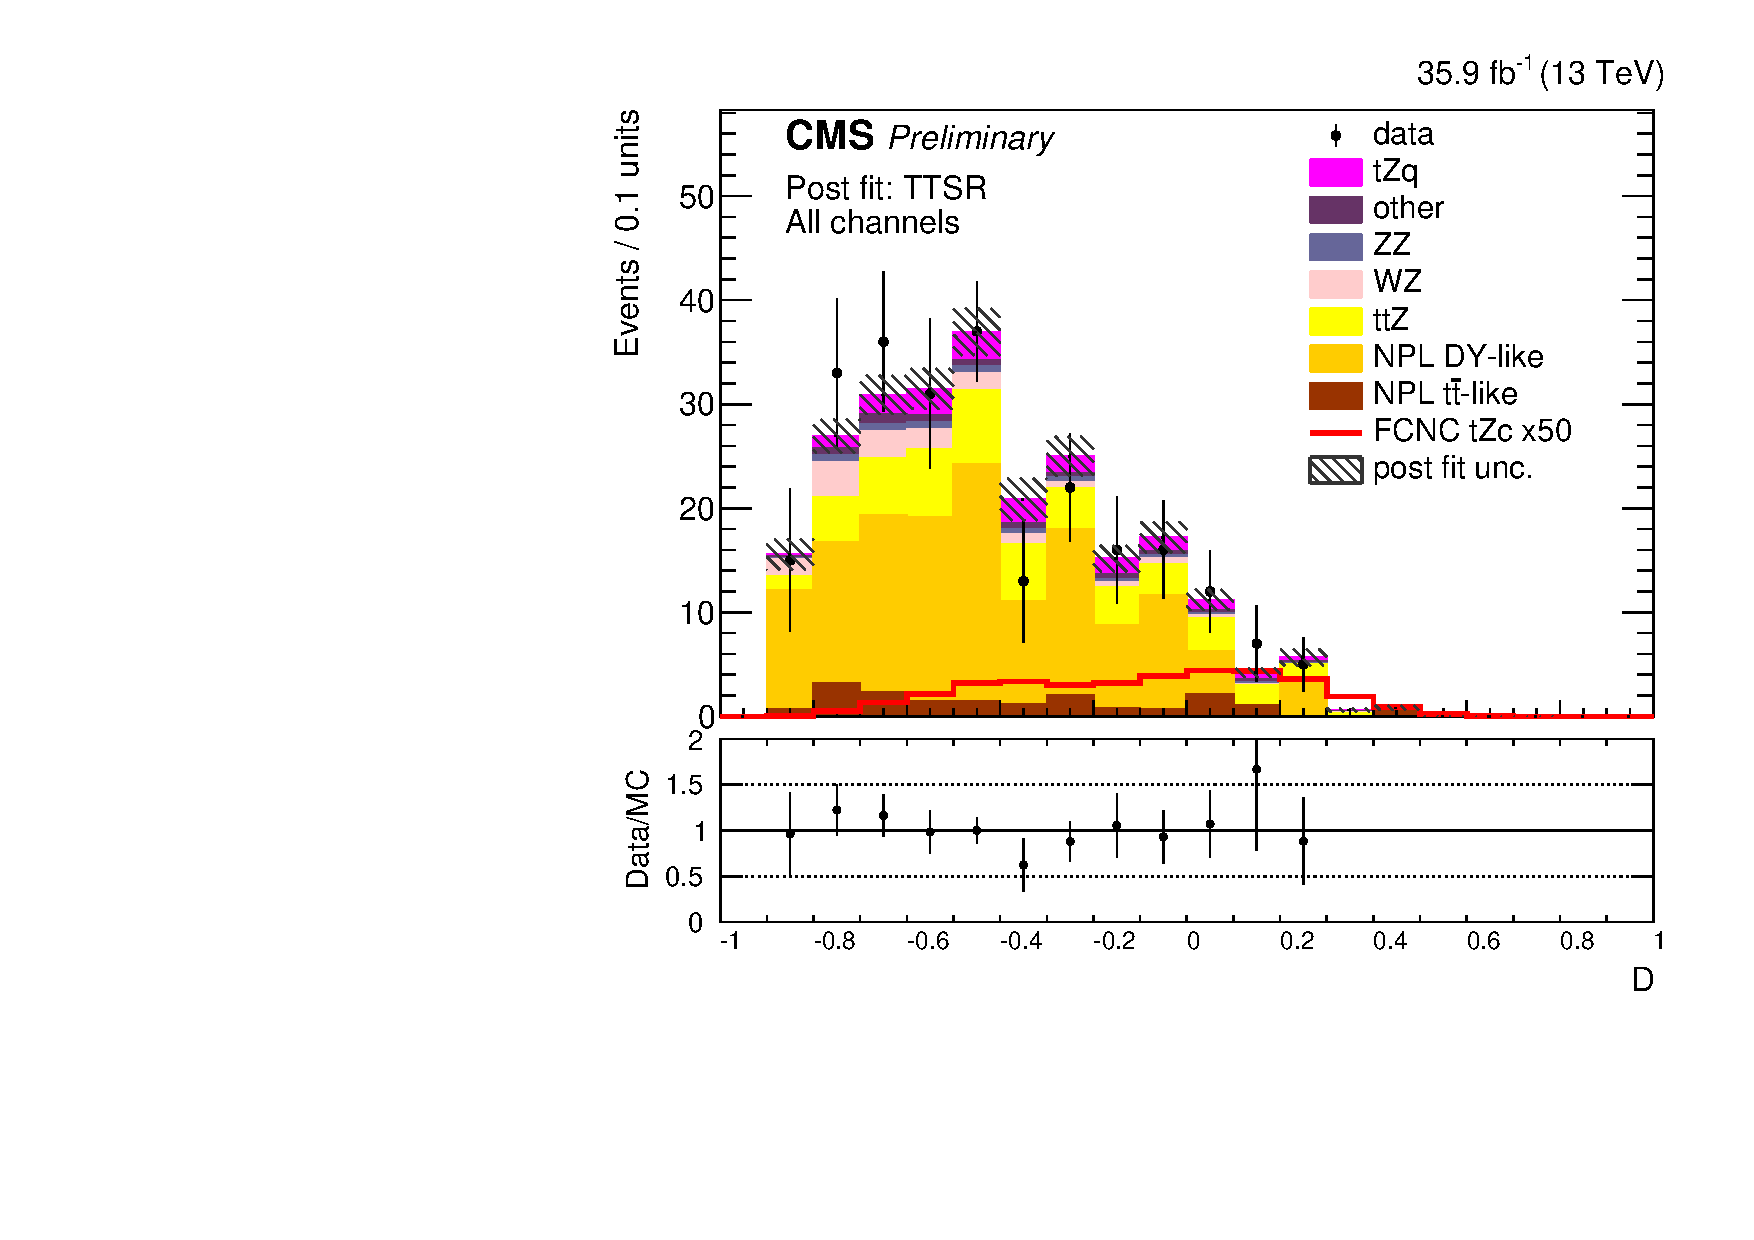
\includegraphics[width=0.45\textwidth]{figures/CMS-PAS-TOP-17-017_Figure_003-b}\\
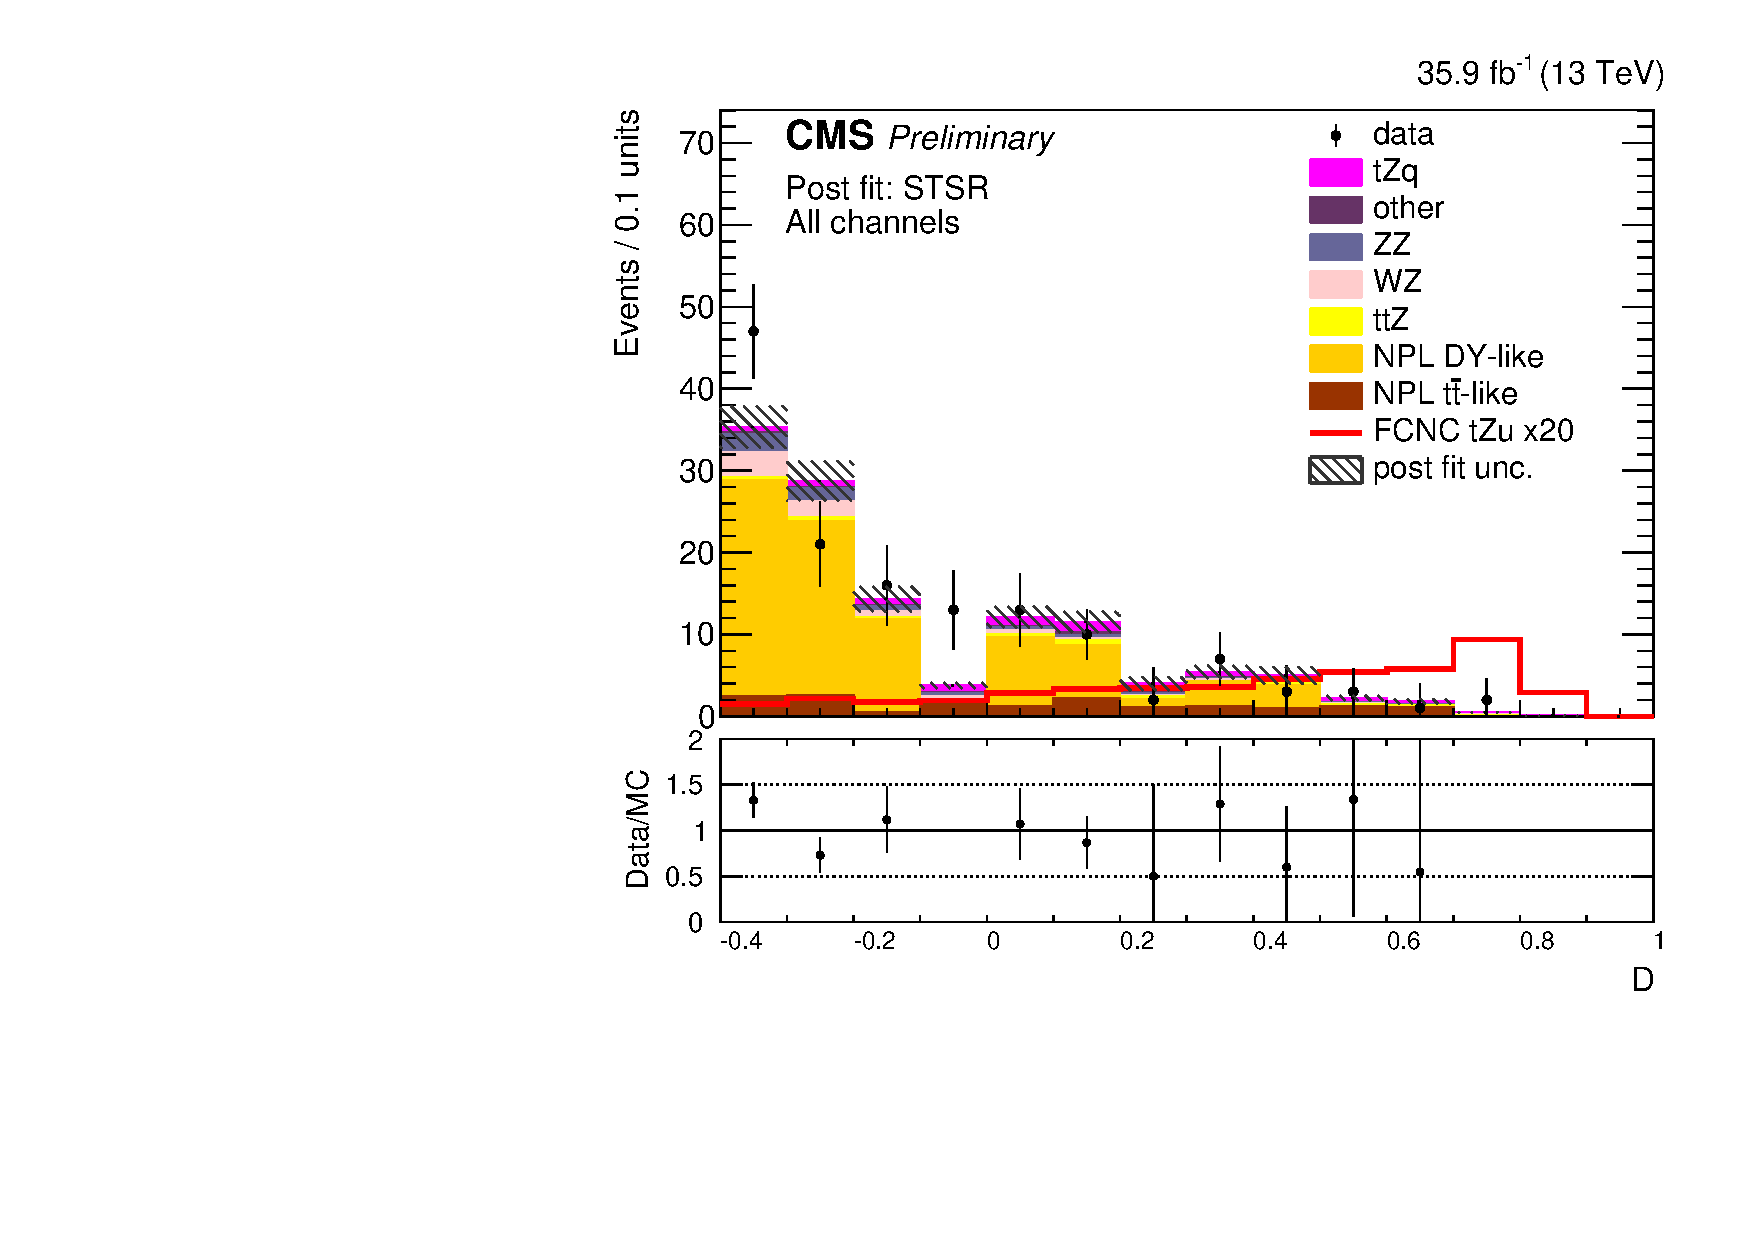
\includegraphics[width=0.45\textwidth]{figures/CMS-PAS-TOP-17-017_Figure_003-c}
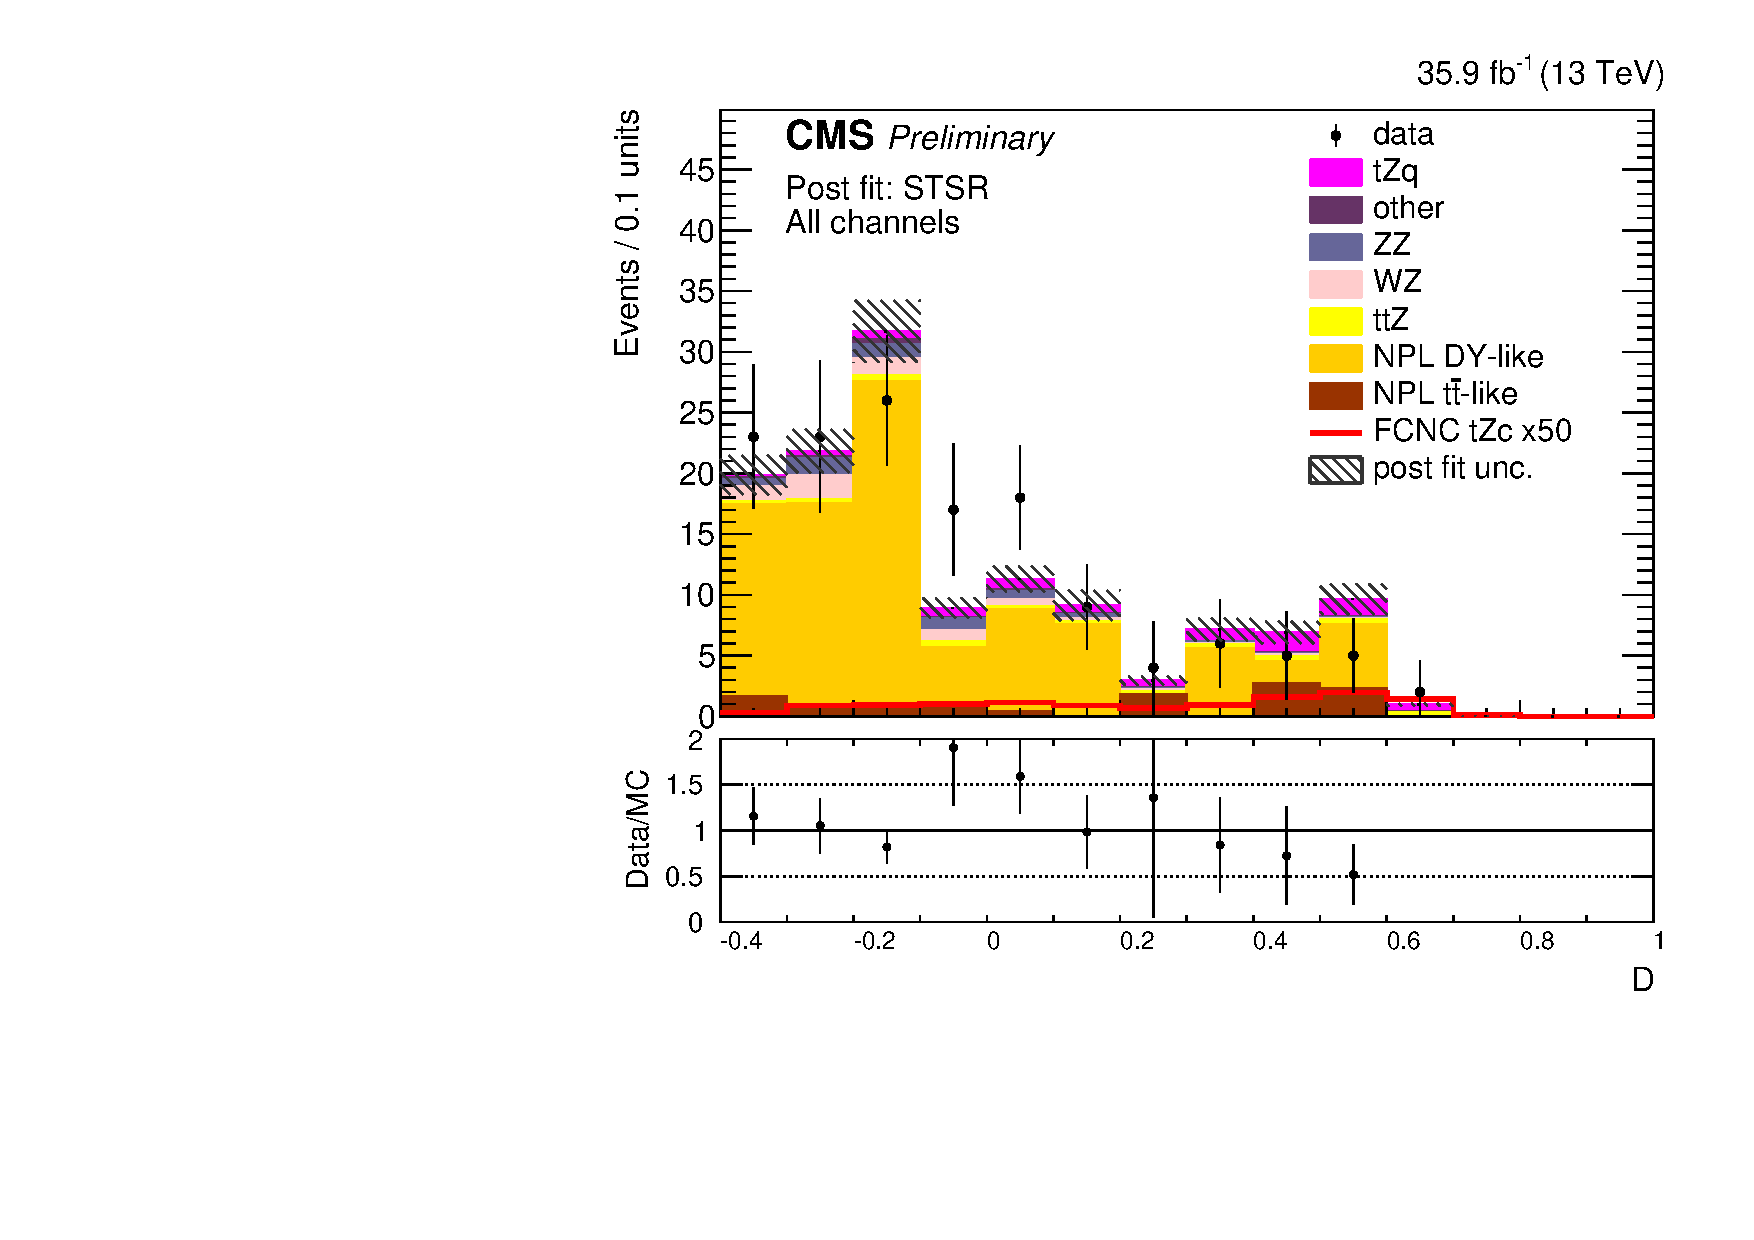
\includegraphics[width=0.45\textwidth]{figures/CMS-PAS-TOP-17-017_Figure_003-d}
\caption{
  The discriminating variable distribution after the fit for all different
  leptonic channels. Upper left: top quark pair tZu; upper right: top quark pair
  tZc; lower left: single top quark tZu; lower right: single top quark tZc.
}
\label{fig:TOP-17-017_Figure_003}
\end{figure}


\begin{figure}[htb]
\centering
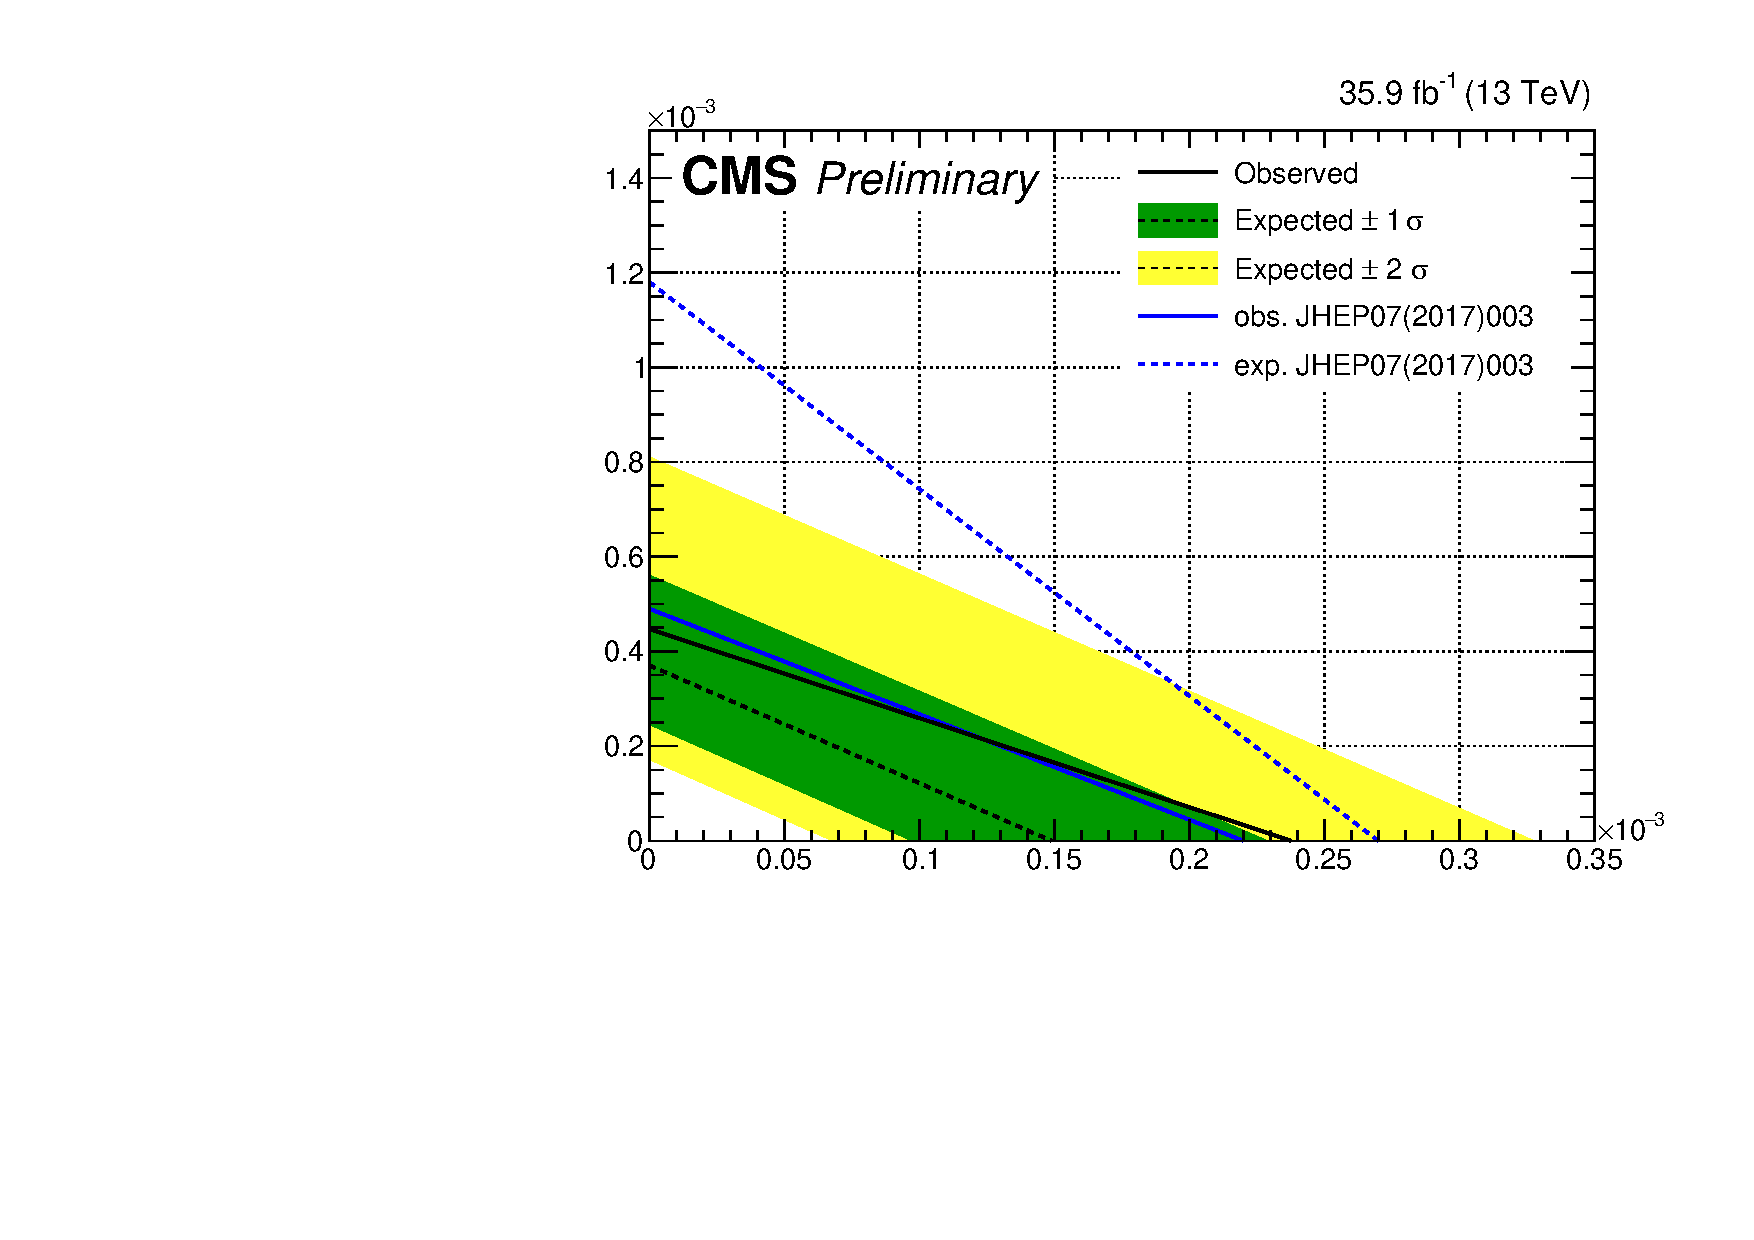
\includegraphics[width=0.45\textwidth]{figures/CMS-PAS-TOP-17-017_Figure_007-a}
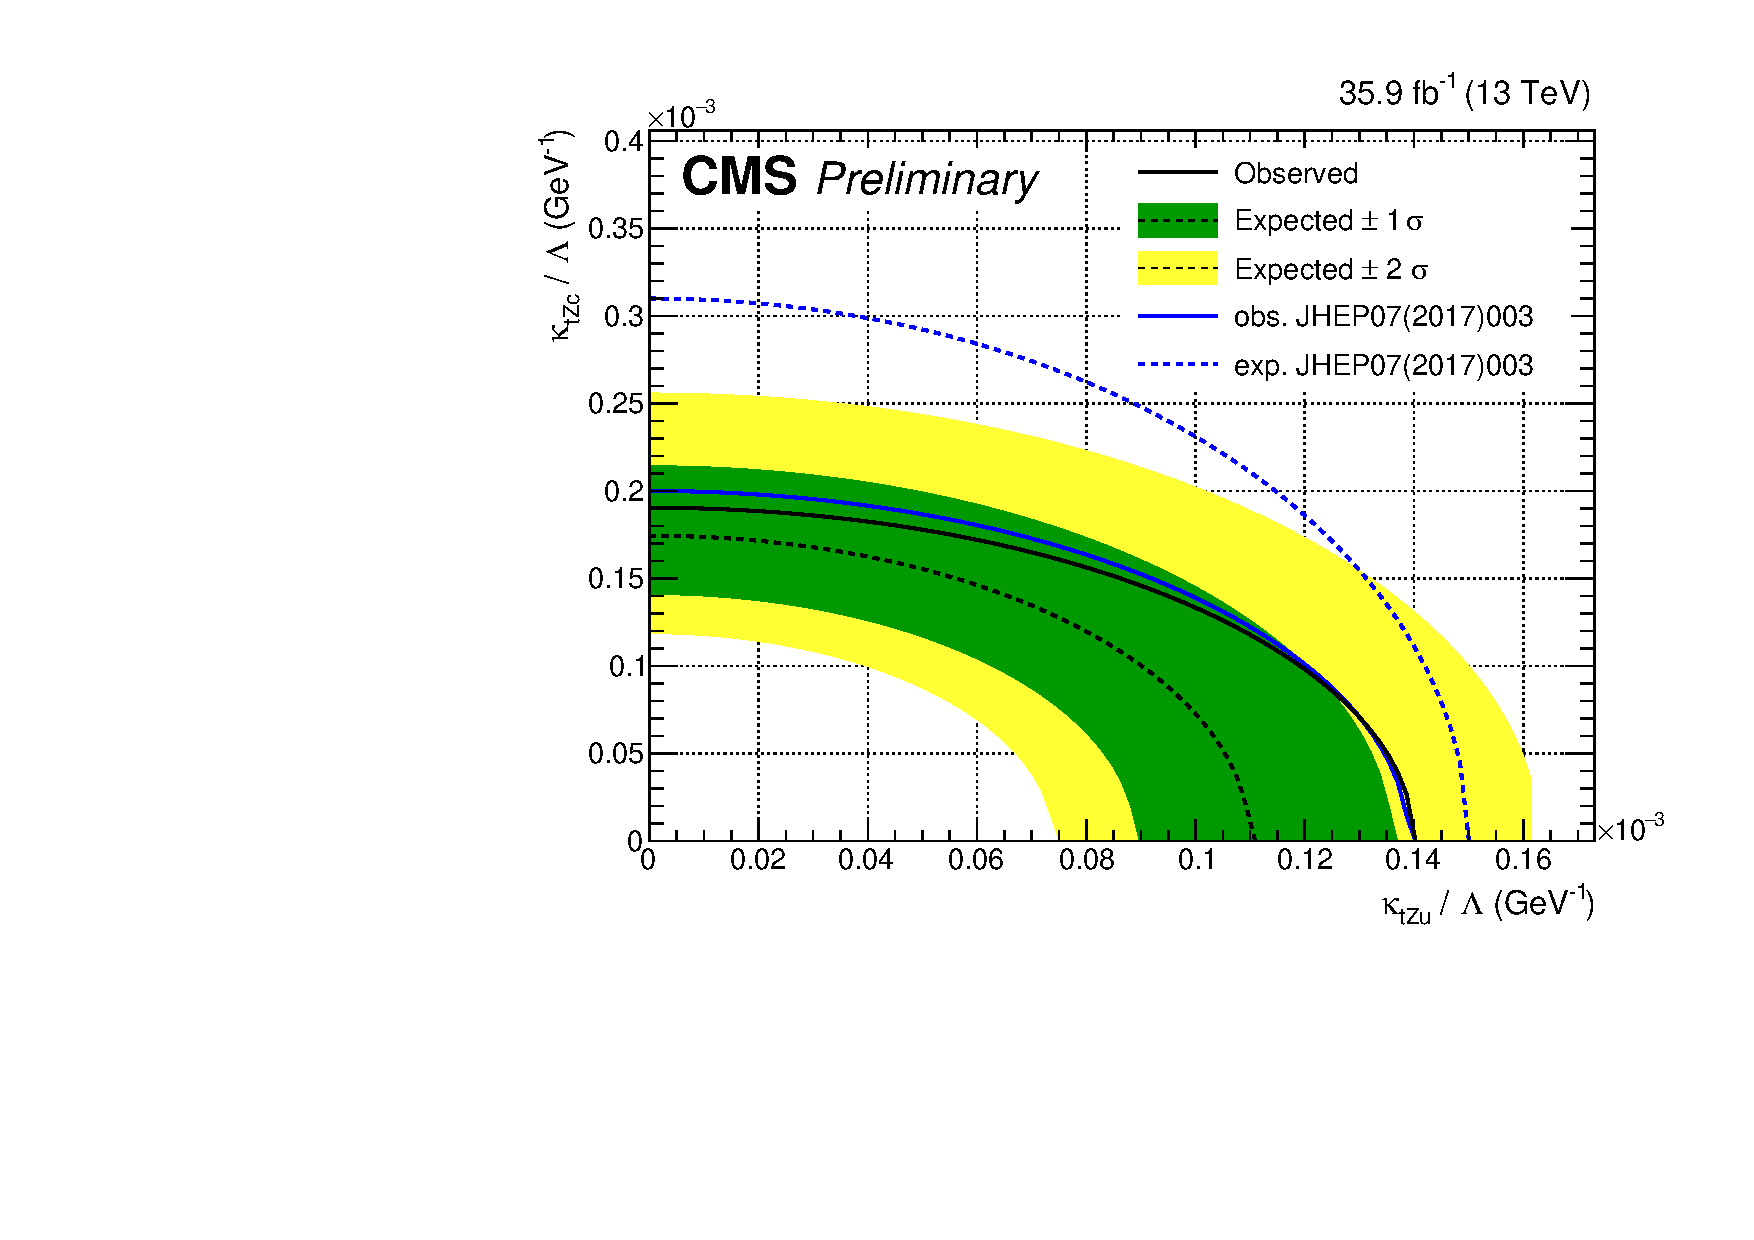
\includegraphics[width=0.45\textwidth]{figures/CMS-PAS-TOP-17-017_Figure_007-b}
\caption{
  Exclusion regions at 95\% CL on the FCNC branching fractions (left) and
  couplings (right) in the 2D plane of both the tZu and tZc variables. The CMS
  8 TeV observed (expected) limit is given with a blue line (dashed line).
}
\label{fig:TOP-17-017_Figure_007}
\end{figure}


%-------------------------------------------------------------------------------
\section{FCNC in ${\rm tH \to bb}$}
%-------------------------------------------------------------------------------

\cite{top-17-003}
\ref{fig:TOP-17-003_Figure_002}
\ref{fig:TOP-17-003_Figures_006-007}


\begin{figure}[htb]
\centering
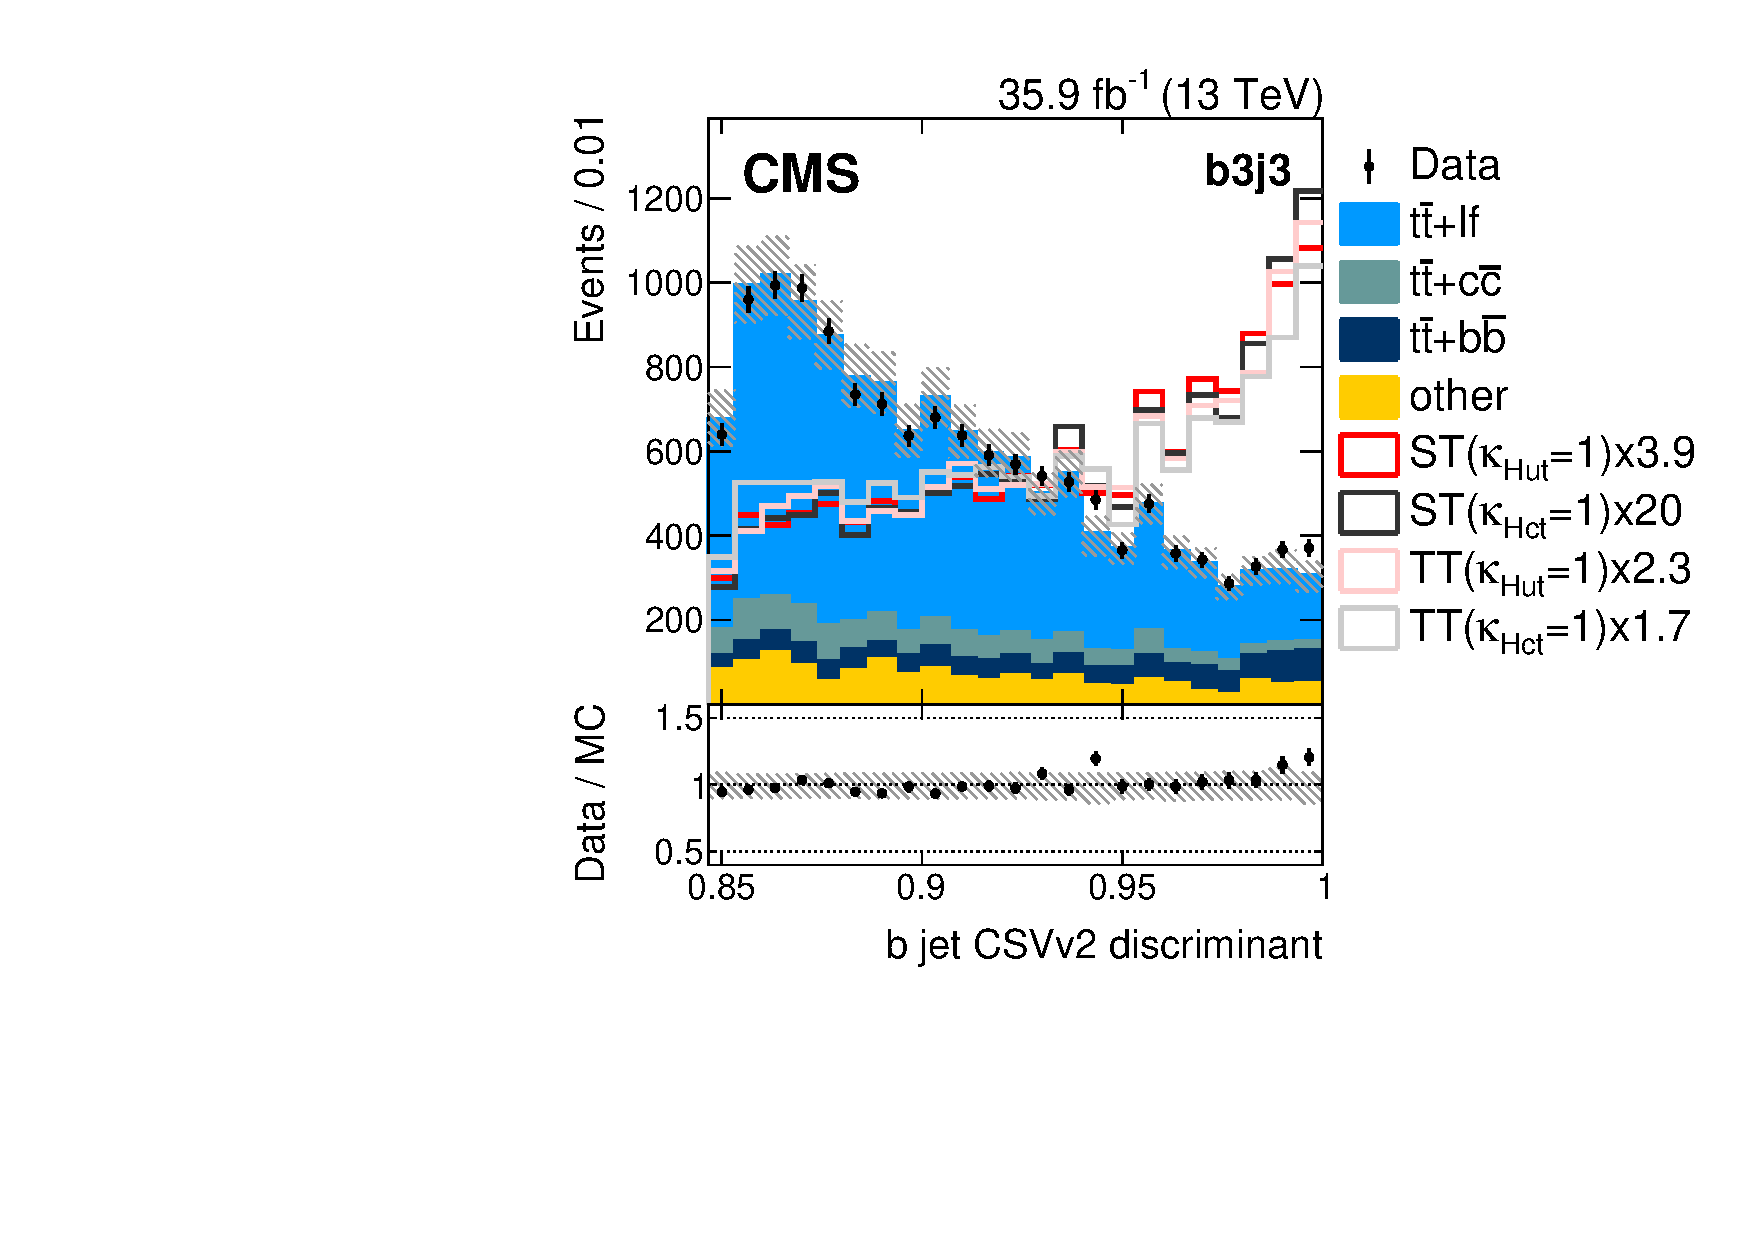
\includegraphics[width=0.45\textwidth]{figures/CMS-TOP-17-003_Figure_002-b}
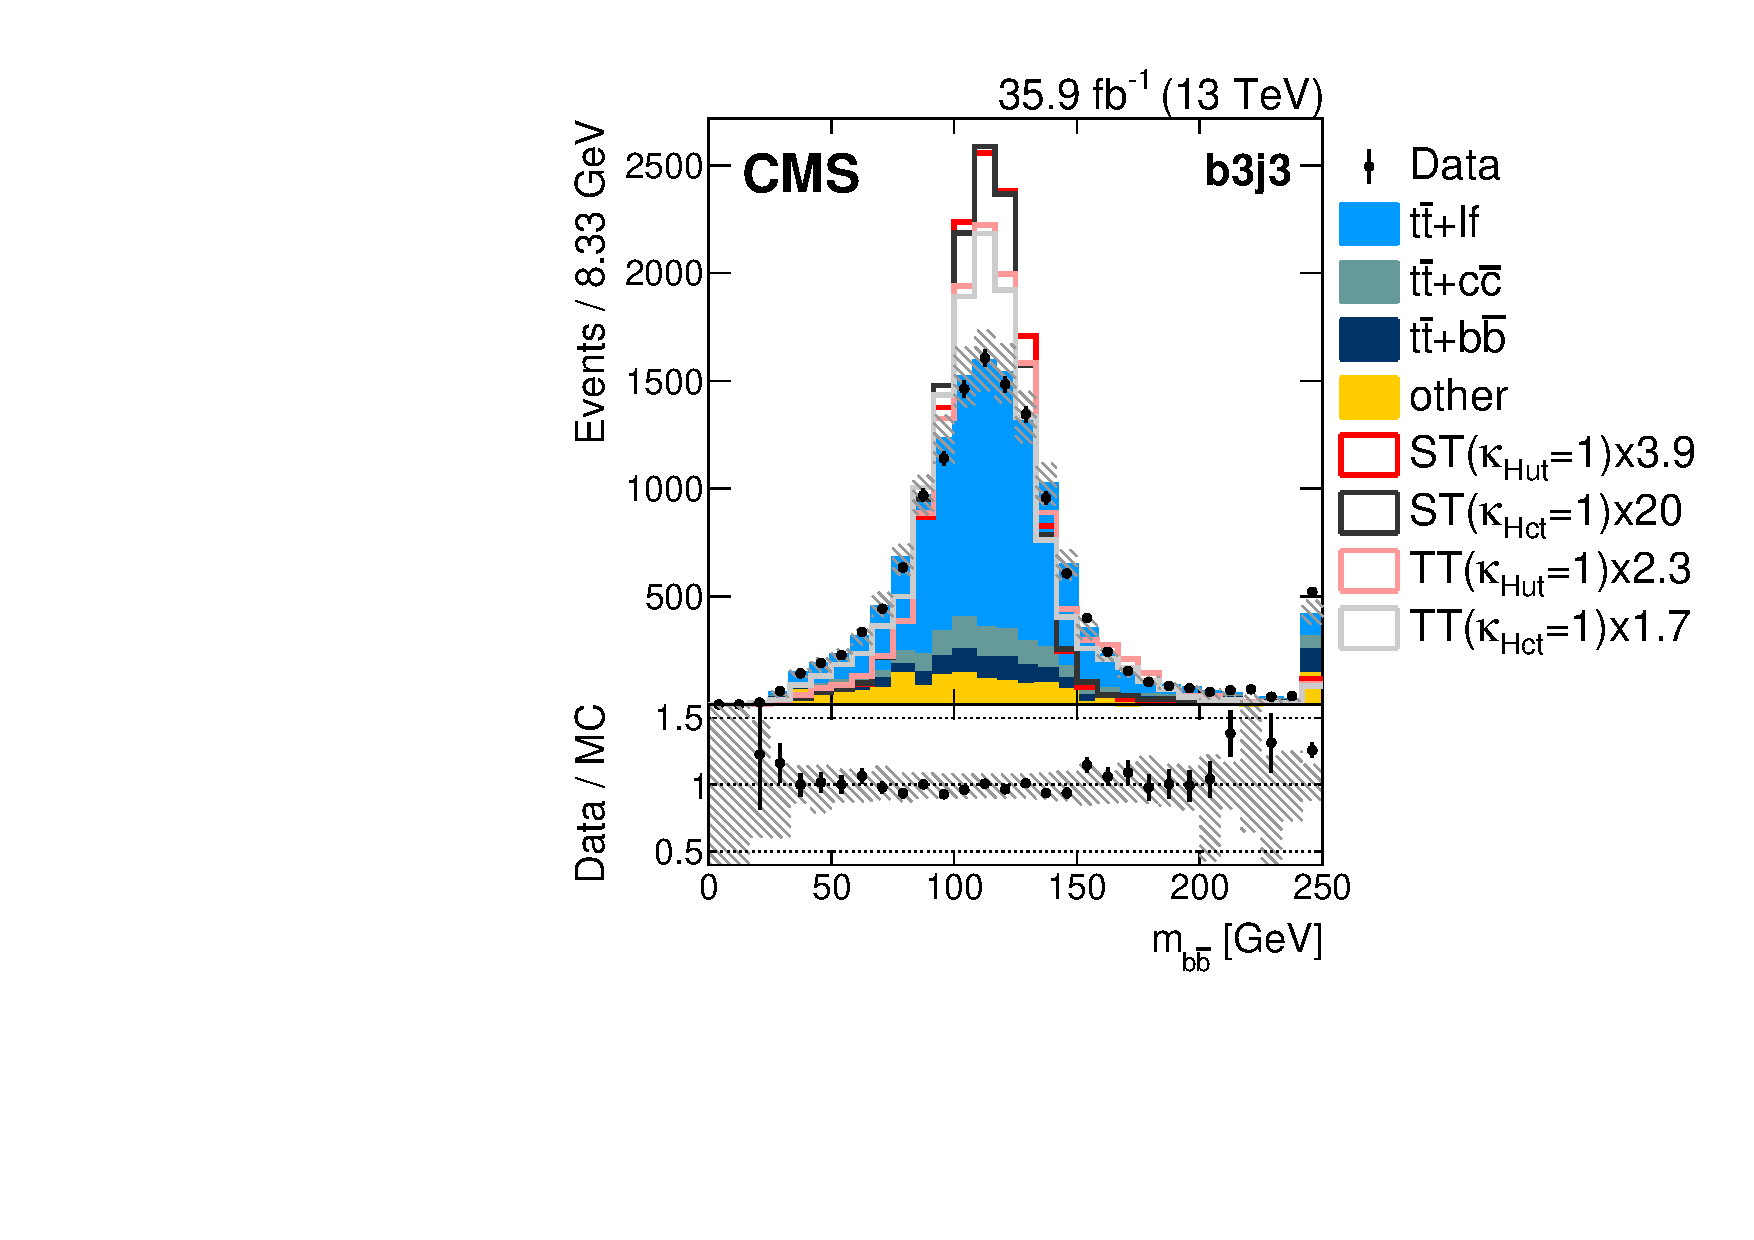
\includegraphics[width=0.45\textwidth]{figures/CMS-TOP-17-003_Figure_002-c}
\caption{
  Comparison between data and simulation for some of the most discriminating BDT
  input variables in the category with three jets, all of them b-tagged: CSV
  discriminant value for one of the reconstructed b jets assigned to Higgs boson
  decay (left), and reconstructed invariant mass of two b jets associated with
  the Higgs boson decay (right).
}
\label{fig:TOP-17-003_Figure_002}
\end{figure}


\begin{figure}[htb]
\centering
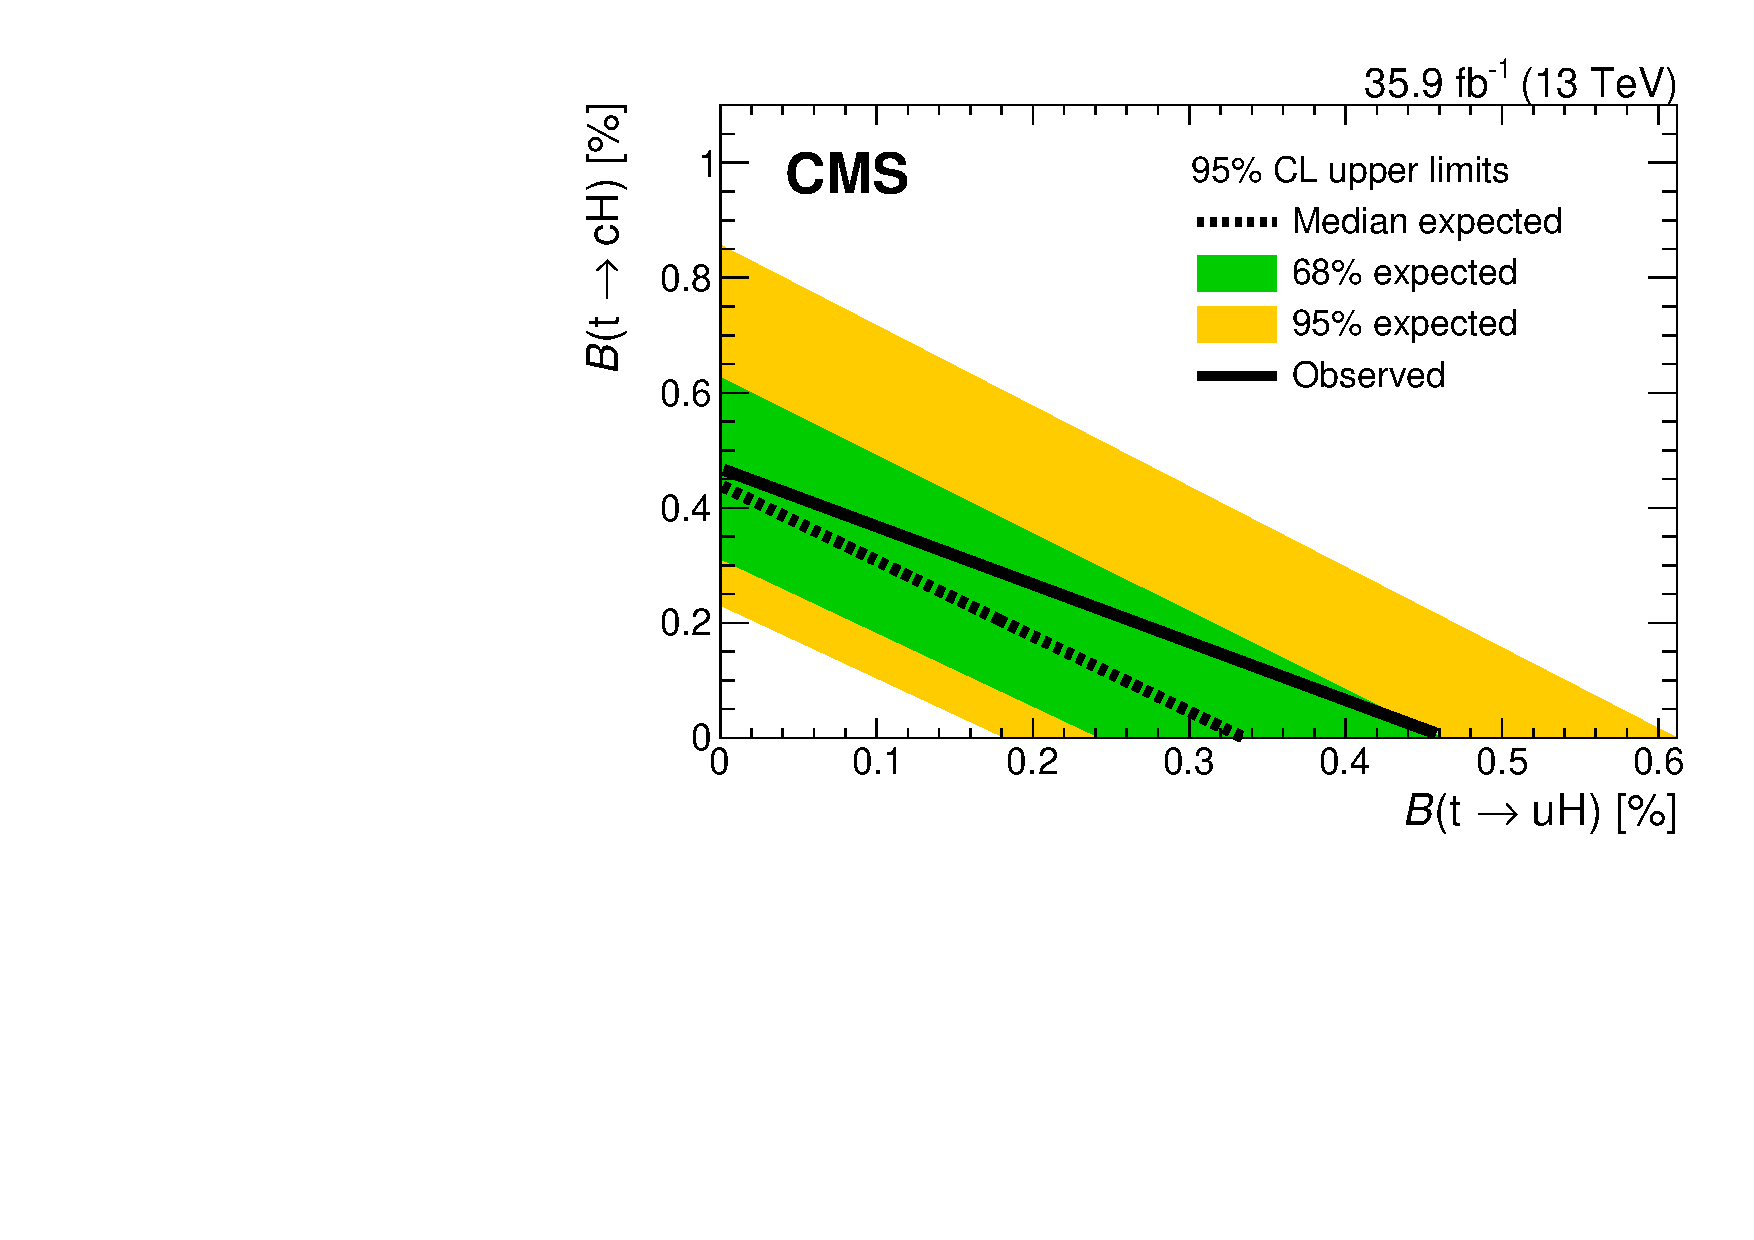
\includegraphics[width=0.3\textwidth]{figures/CMS-TOP-17-003_Figure_006}
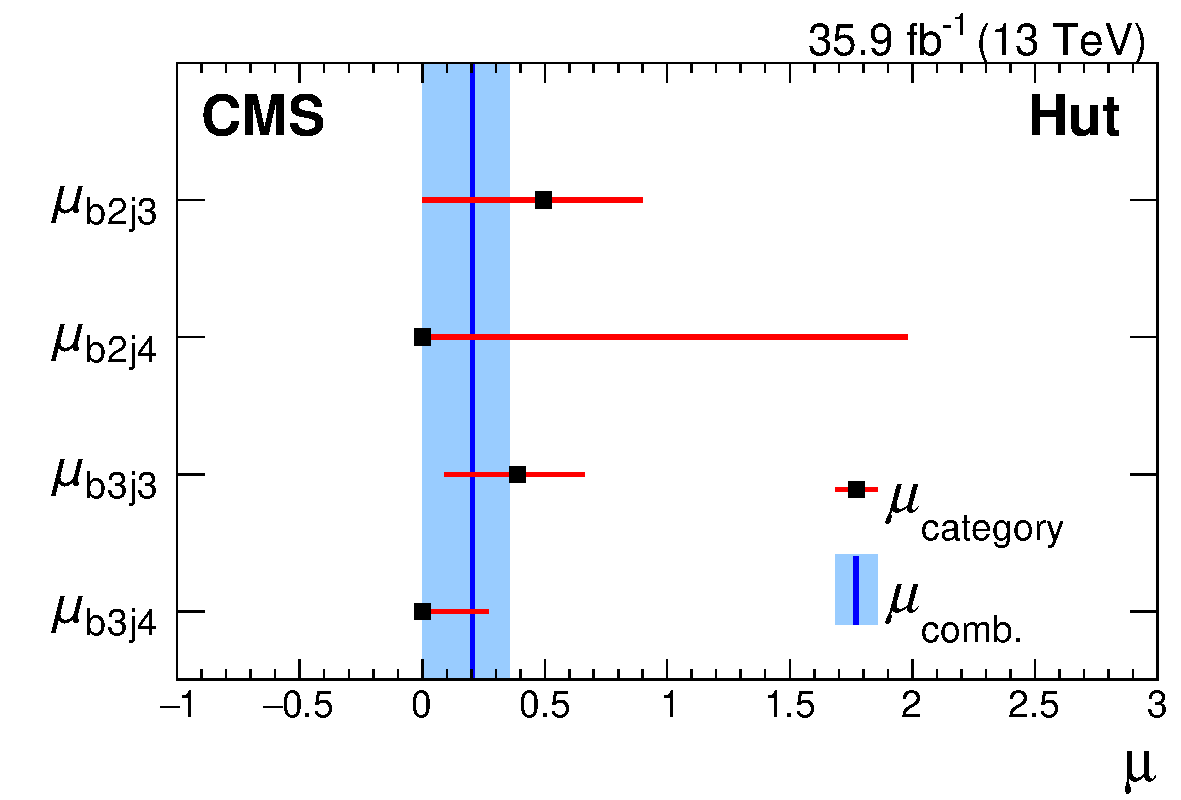
\includegraphics[width=0.3\textwidth]{figures/CMS-TOP-17-003_Figure_007-a}
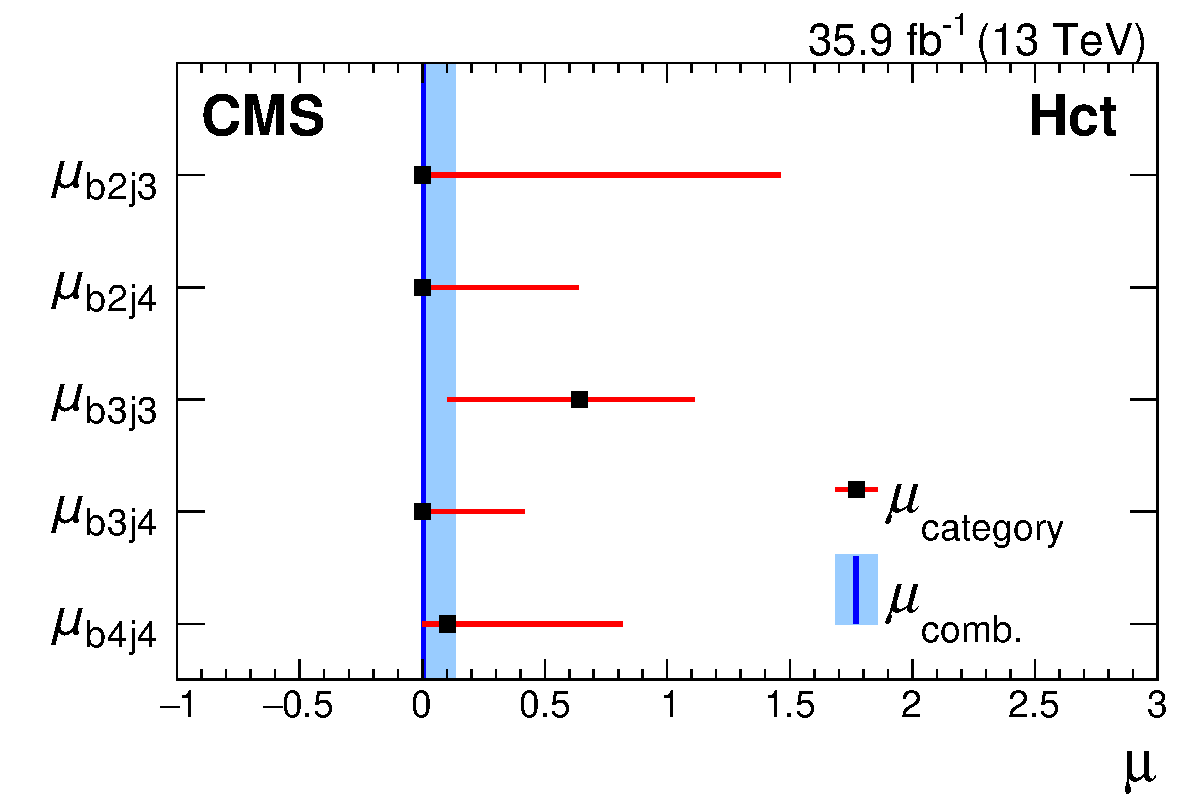
\includegraphics[width=0.3\textwidth]{figures/CMS-TOP-17-003_Figure_007-b}
\caption{
  Upper limits on ${\cal B}({\rm t \to uH})$ and ${\cal B}({\rm t \to cH})$ at
  95 \% CL (left), and the best fit signal strength for Hut (center) and Hct
  (right), which is restricted to positive values in the fit.
}
\label{fig:TOP-17-003_Figures_006-007}
\end{figure}


%-------------------------------------------------------------------------------
\section{Angular observables in ${\rm B^+ \to K^+\mu\mu}$}
%-------------------------------------------------------------------------------

\cite{bph-15-001}


%-------------------------------------------------------------------------------
\section{Angular observables in ${\rm B^0 \to K^{*0}\mu\mu}$}
%-------------------------------------------------------------------------------

\cite{bph-15-008}


%-------------------------------------------------------------------------------
\section{Conclusions}
%-------------------------------------------------------------------------------

To be filled.


%-------------------------------------------------------------------------------
\begin{thebibliography}{99}
%-------------------------------------------------------------------------------

\bibitem{top-17-017}
  CMS Collaboration,
  \emph{Search for flavour changing neutral currents in top quark production and decays with three-lepton final state using the data collected at $\sqrt{s} = 13~{\rm TeV}$},
  https://cds.cern.ch/record/2292045, CMS-PAS-TOP-17-017.
\bibitem{top-17-003}
  CMS Collaboration,
  \emph{Search for the flavor-changing neutral current interaction of the top quark and the Higgs boson which decays into a pair of b quarks at $\sqrt{s} = 13~{\rm TeV}$},
  \emph{accepted for publication in JHEP}
  https://cds.cern.ch/record/2296416, CERN-EP-2017-309
  [{\tt hep-ex/1712.02399}].
\bibitem{bph-15-001}
  CMS Collaboration,
  \emph{Angular analysis of the decay ${\rm B^+ \to K^+\mu^+\mu^-}$ at ${\rm \sqrt{s} = 8~TeV}$},
  https://cds.cern.ch/record/2621370 CERN-EP-2018-125
  [{\tt hep-ex/1806.00636}].
\bibitem{bph-15-008}
  CMS Collaboration,
  \emph{Measurement of angular parameters from the decay ${\rm B^0 \to K^{*0}\mu^+\mu^-}$ at ${\rm \sqrt{s} = 8~TeV}$},
  https://cds.cern.ch/record/2287571, CERN-EP-2017-240
  [{\tt hep-ex/1710.02846}].  
\end{thebibliography}

\end{document}
(https://pos.sissa.it/cgi-bin/reader/contribution.cgi?id=PoS(MC2000)002).
